\section{Ray marching}
\begin{frame}{Algoritmos basados en rayos}
En realidad esta es un familia de algoritmos, los mas importantes son:

\begin{itemize}
    \item \href{https://en.wikipedia.org/wiki/Ray_casting}{Ray Casting:} El primero en ser desarrollado. Consiste en lanzar un rayo por cada pixel del viewport. Para ver donde interfecta la escena.
    \item \href{https://en.wikipedia.org/wiki/Ray_tracing_(graphics)}{Ray Tracing:} Una generalización donde cada vez que se intersecta la escena, se calcula el angulo de reflexión y se continua siguiendo el rayo, hasta cumplir algún criterio de paro.
    \item \href{https://en.wikipedia.org/wiki/Ray_marching}{Ray Marching:} Un caso particular del anterior. Una forma de usar las sdf, para acelerar el camino de los rayos de manera recursiva. Éste es el mas usado en Shadertoy.
    \item \href{https://en.wikipedia.org/wiki/Path_tracing}{Path Tracing:} En vez de lanzar un rayo, se lanzan varios rayos a varios ángulos usando el método de Monte Carlo.
\end{itemize}

\end{frame}

\begin{frame}{El rayo}
\begin{block}{Rayo}
Un rayo es el semisegemento de linea $\mathbf{r}(s) = \mathbf{o} + s  \mathbf{d}$, donde $s \in \mathbb{R}^{+}$ es un escalar no negativo, $\mathbf{o}$ es un punto en $\mathbb{R}^3$ y $|\mathbf{d}| = 1$ un vector unitario en $\mathbb{R}^3$.

\end{block}

\begin{columns}
\column[t]{0.5\textwidth}
\begin{itemize}
    \item $\mathbf{o}$ es el origen del rayo.
    \item $\mathbf{d}$ es la dirección del rayo.
    \item $s$ es el parámetro.
\end{itemize}    
\column[t]{0.5\textwidth}
\begin{figure}[htp]
    \centering
    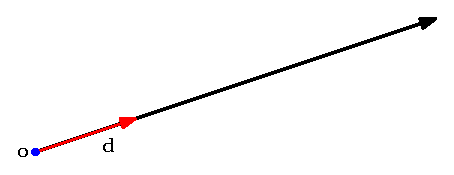
\includegraphics[width=0.6\textwidth]{img/ray.eps}    
\end{figure}
\end{columns}
\end{frame}

\begin{frame}{Ray Marching}
Es una técnica para hacer un avance adaptativo de los rayos.
\begin{enumerate}
    \item En el punto actual del rayo calcula la distancia $d$ del punto con respecto a la escena.
    La \emph{distancia} de la escena, es la mínima de todas las sdfs a las figuras en la escena.
    \item Si $d$ es menor que un cierto $\epsilon$, termina y reporta que hay una colisión con la escena.
    \item Si $d$ es mayor que un cierto valor frontera termina y di que no hay colisión.
    \item Avanza el rayo en $d$ unidades, y repite desde 1.
\end{enumerate}
Esta técnica solo se puede usar si\ldots
\begin{itemize}
    \item Definimos la escena por medio de sdfs.
    \item El rayo tiene un vector de dirección unitario.
    \item Las sdf están bien definidas:
    \begin{itemize}
        \item Continuas.
        \item La distancia esta en la misma dimensión que la escena.
    \end{itemize}    
\end{itemize}

\end{frame}

\begin{frame}{Ray Marching: una imagen}

\begin{itemize}
    \item En la practica se pone un numero máximo de pasos como criterio extra de paro.
\end{itemize}    

\begin{figure}[htp]
    \centering
    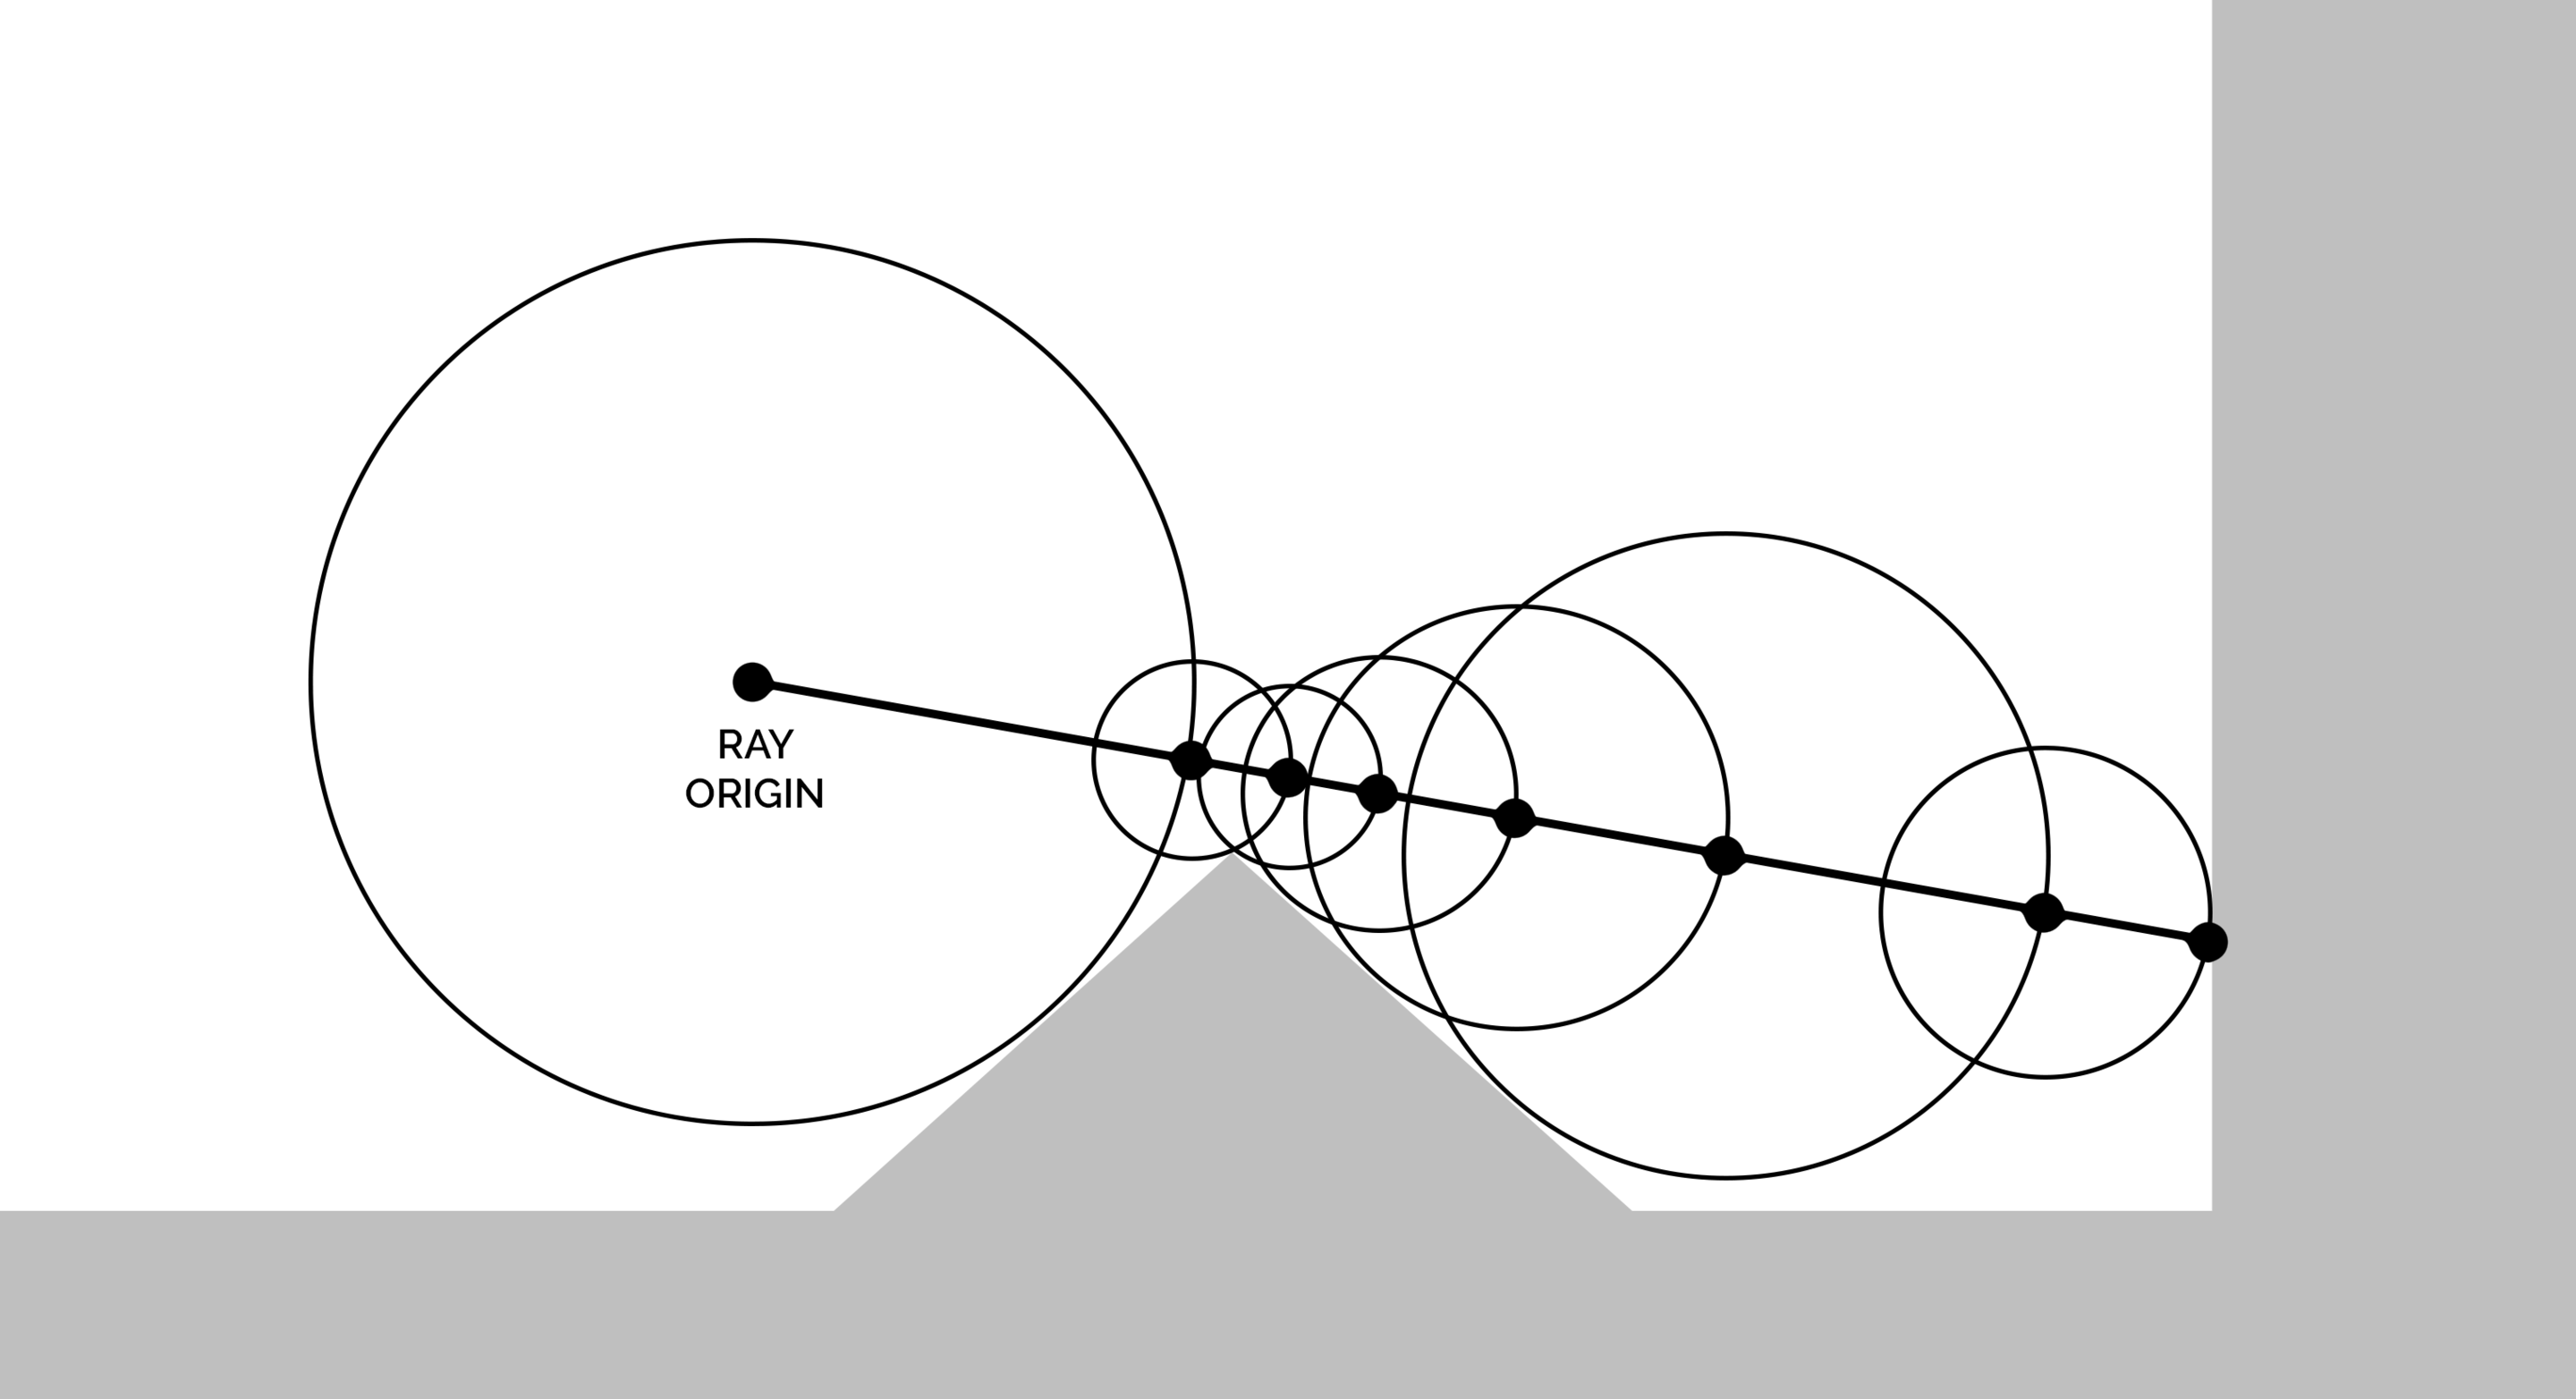
\includegraphics[width=0.6\textwidth]{img/rayMarch}    
\end{figure}

Hay un \href{https://www.shadertoy.com/view/4dSfRc}{ejemplo} para visualizar la técnica en ShaderToy mismo.

\end{frame}

\begin{frame}[fragile]{Ray Marching: en código}
\begin{listing}
\begin{minted}{glsl}
float rayMarch(Ray ray, float start, float end) {
  float depth = start;

  for (int i = 0; i < MAX_MARCHING_STEPS; i++) {
    vec3 position = ray.origin + depth * ray.direction;
    float d = sdScene(position);
    depth += d;
    if (d < PRECISION || depth > end) break;
  }

  return depth;
}
\end{minted}
\end{listing}

\end{frame}

\begin{frame}{Visualizar en 3D}
\begin{itemize}
    \item Para no ver todo de un color plano en 3D, necesitamos hacer shading.
    \item Para hacer shading, necesitamos (entre otras cosas), la normal $\mathbf{n}$ a la superficie en el punto de contacto.
    \item Podemos utilizar la misma sdf, para calcular el gradiente $\nabla$ de la figura. El gradiente es una buena aproximación a la normal: $\nabla \approx \mathbf{n}$.
\end{itemize}
$$\nabla (f(\mathbf{x})) = \begin{pmatrix}
f(x + \epsilon, y, z) - f(x - \epsilon, y, z)\\
f(x, y + \epsilon, z) - f(x, y - \epsilon, z)\\
f(x, y, z + \epsilon) - f(x, y, z - \epsilon)
\end{pmatrix}$$
Donde $f(\mathbf{x})$ es una sdf y $\epsilon$ un numero positivo muy pequeño.
\begin{itemize}
    \item Finalmente, si definimos una fuente de luz, con una posición al que el vector $\mathbf{l}$ apunta.
    \item Una forma muy sencilla de shading puede ser: $\mathbf{c} = \max(\mathbf{k}_d (\mathbf{l} \cdot \mathbf{n}), \mathbf{0})$.
    \item Donde $\mathbf{c}$ es el color resultante y $\mathbf{k}_d$ es el color predominante de la superficie.
\end{itemize}
\end{frame}

\begin{frame}{Ejercicio: Esfera usando Ray Marching}
\url{https://github.com/nemediano/tallerShadertoy/tree/main/codigo/Ejercicio4}
\begin{columns}
\column[t]{0.5\textwidth}
     \begin{itemize}
         \item De momento, usa solo una esfera en la escena.
         \item Trata de definir tu cámara, la esfera y una fuente de luz, en lugares sencillos respecto al origen.
         \item De momento usa la reflexión difusa, para que puedas visualizar al esfera.
         \item Puedes usar el código de comienzo de la escena para empezar.
     \end{itemize}
\column[t]{0.5\textwidth}
        \begin{figure}[htb]
            \centering
            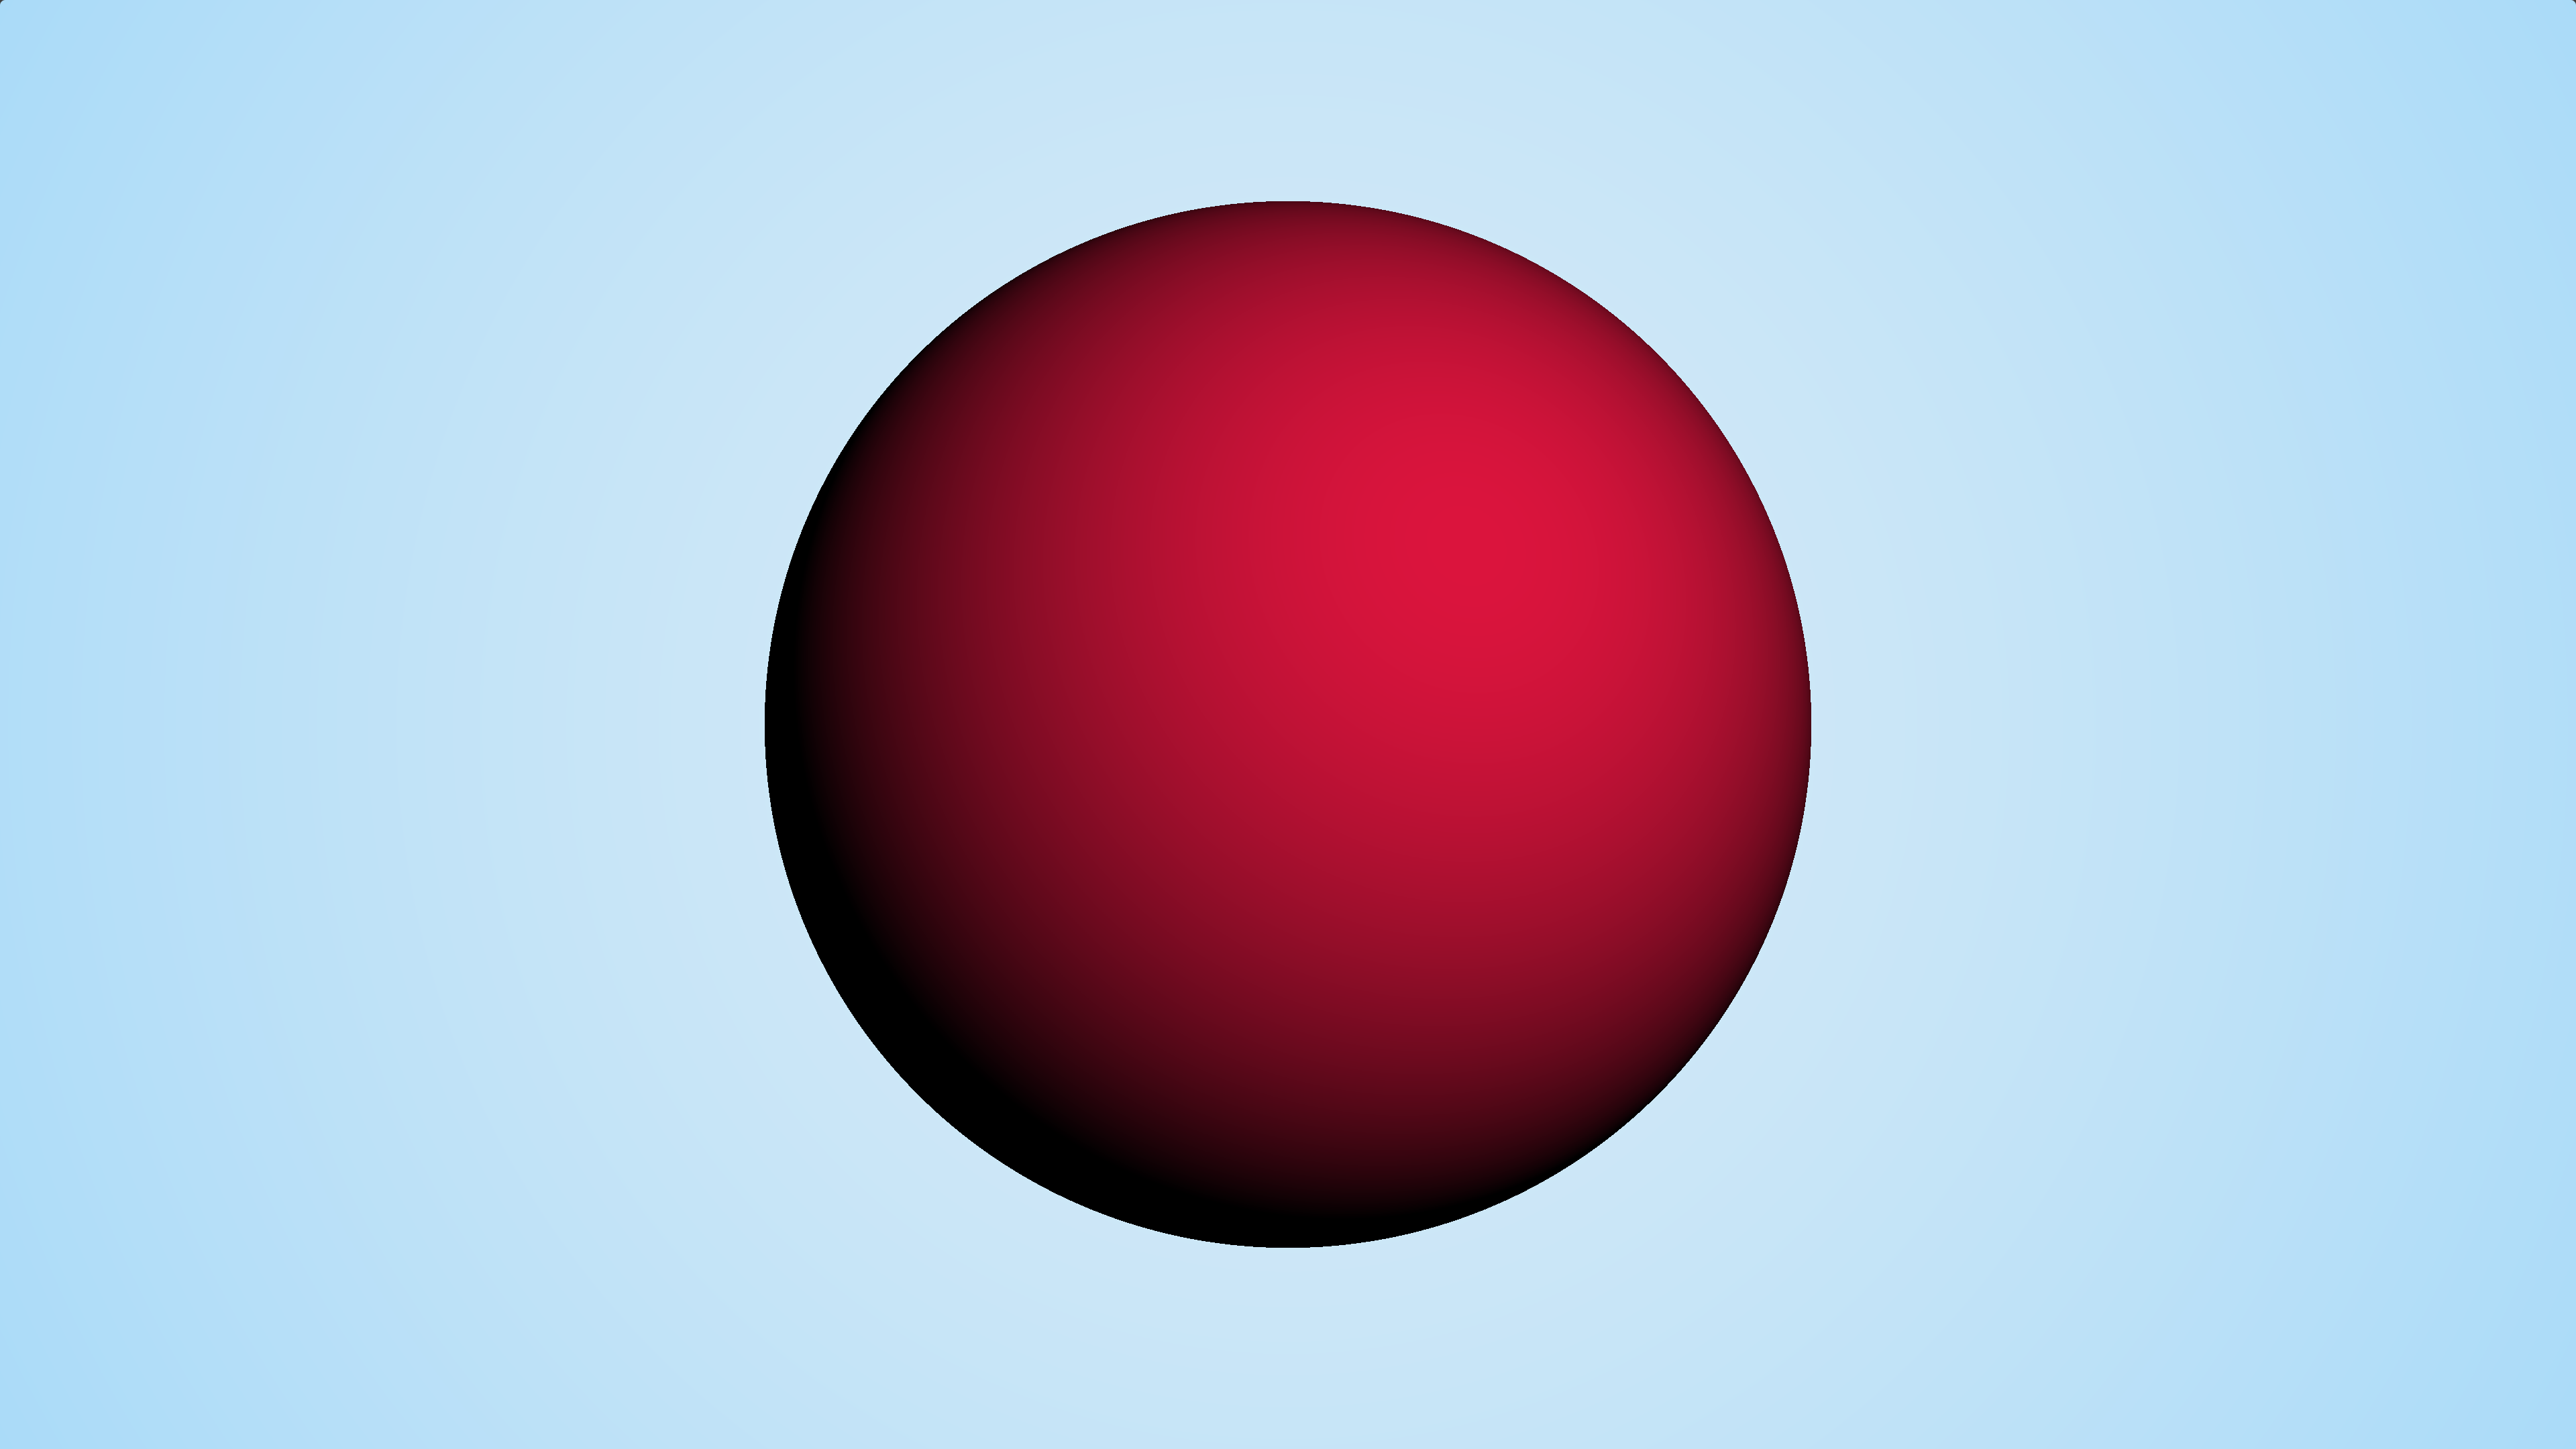
\includegraphics[width=0.6\textwidth]{img/Ejer/Ejer4}
        \end{figure}
\end{columns}
\end{frame}

\begin{frame}{¿Qué mas podemos añadir?}

En lo que resta del taller vamos a añadir algunas cosas al ejemplo de Raymarching:

\begin{enumerate}
    \item Como manejar una escena con varios objetos.
    \item Como hacer un modelo de cámara mas robusto.
    \item El modelo de iluminación de Blin-Phong.
    \item \href{https://en.wikipedia.org/wiki/Constructive_solid_geometry}{Constructive solid geometry} gracias a las sdf.
\end{enumerate}

\end{frame}

\subsection{Escena con mas de un objeto}
\begin{frame}[fragile]{Generalizar la escena para varios objetos}
Actualmente, la escena esta definida por una sola sdf.
Para hacer el código mas general hay varios métodos.
Aquí solo voy a explicar uno de ellos.

\begin{itemize}
    \item Definir una estructura mas general que represente un punto en la escena.
    \item De momento contiene un escalar que representa la distancia del punto sobre el rayo.
    \item Para demostrar la utilidad vamos a incluir un campo extra (el color).
\end{itemize}

\begin{listing}
\begin{minted}{glsl}
struct ScenePoint {
  float dist;
  vec3 color;
};
\end{minted}
\end{listing}

\end{frame}

\begin{frame}[fragile]{Mas detalles\ldots}
\begin{itemize}
    \item La función \mintinline{glsl}{sdScene} debería regresar ahora un \mintinline{glsl}{ScenePoint}.
    \item Por supuesto, esto requiere cambiar \mintinline{glsl}{calcNormal}
    \item Y por ultimo, también cambiar \mintinline{glsl}{RayMarch} para regresar un \mintinline{glsl}{ScenePoint}. 
\end{itemize}

\begin{block}{¿Qué necesitamos saber de un punto en la escena?}
    \begin{itemize}
        \item Antes, lo único que necesitábamos para identificar un punto en la escena era la distancia a la que debíamos marchar el rayo.
        
        \item Solo le estamos poniendo mas información a ese punto.
    \end{itemize}
\end{block}

\begin{block}{¿Como se manejan varios objetos en la escena?}
    \begin{itemize}
        \item La función \mintinline{glsl}{sdScene} debe de regresar la \alert{distancia mínima} de la distancias a todos los objetos de la escena. 
        
        \item La escena es un objeto formado por todos los objetos que contiene. Por lo tanto, la \say{sdf de la escena} esta definida como la mínima de todas las distancias.
    \end{itemize}
\end{block}
\end{frame}

\begin{frame}[fragile]{Agregando el piso de la escena}
Podemos definir fácilmente la sdf de un semiespcacio ortogonal al eje $y$.
\begin{listing}
\begin{minted}{glsl}
float sdFloor(vec3 position, float floorHeight) {
    return position.y - floorHeight;
}
\end{minted}
\end{listing}
Y podemos definir un color en términos de una posición en el plano $xy$, por ejemplo para crear un patrón de \say{tablero de ajedrez}.
\begin{listing}
\begin{minted}{glsl}
vec3 getCheckboardPattern(vec2 coords, vec3 colorEven, vec3 colorOdd) {
    float alpha = mod(floor(coords.x) + floor(coords.y), 2.0);
    return mix(colorEven, colorOdd, alpha);
}
\end{minted}
\end{listing}

\end{frame}

\begin{frame}[fragile]{Ejemplo de sdf con varios objetos}
\begin{listing}
\begin{minted}{glsl}
ScenePoint sdScene(vec3 position) {
  ScenePoint closestShape;
  // Closest shape is the first shape (the floor)
  closestShape.dist = sdFloor(position, -1.0);
  closestShape.color = getCheckboardPattern(position.xz, vec3(1.0), vec3(1.4));
  // Now test the second shape (a box)
  float testDistance = sdBox(position, vec3(1.5, 0.0, 0.0), vec3(1.0));
  // If this shape is closer, update closest shape
  if (testDistance < closestShape.dist) {
    closestShape.dist = testDistance;
    closestShape.color = DarkSeaGreen;
  }

  return closestShape;
}
\end{minted}
\end{listing}
\end{frame}

\subsection{Un modelo de cámara}

\begin{frame}{Un modelo de cámara típico}
En CG, la cámara esta definida con dos matrices:
\begin{enumerate}
  \item La de \alert{vista}: Que contiene la \href{https://en.wikipedia.org/wiki/Pose_(computer_vision)}{pose} de la cámara.
  \item La de \alert{proyección}: Que define el volumen de visión de la cámara.
\end{enumerate}
\begin{itemize}
   \item Una \say{pose} es una posición, en el espacio junto con una orientación (dirección).
   \begin{itemize}
     \item Típicamente, se usan un punto en $\mathbb{R}^3$ y un \href{https://en.wikipedia.org/wiki/Quaternion}{cuaternión}. Por lo que tiene 7 grados de libertad.
     \item Piensa en ella como posicionar tu cámara usando un \href{https://en.wikipedia.org/wiki/Tripod_(photography)}{tripié}
   \end{itemize}
   \item Cuando decimos proyección, generalmente queremos decir \href{https://en.wikipedia.org/wiki/3D_projection\#Perspective_projection}{proyección en perspectiva}.
   \begin{itemize}
     \item Se define con una proporción del plano (\emph{aspect ratio}) y dos distancias: la cercana y la lejana.
     \item Piensa en ella como configurar tu cámara: escoger el lente adecuado, ajustar el zoom, etc.
   \end{itemize}
\end{itemize}
\begin{block}{}
 En nuestro caso la proyección esta implícita en el algoritmo de Ray Marching.
 \begin{itemize}
   \item Solo nos hace falta construir la matriz de vista.
 \end{itemize}
\end{block}
\end{frame}

\begin{frame}[fragile]{La pose de la cámara}
Hay varias maneras de definir una pose para nuestra cámara.
\begin{itemize}
    \item No necesitamos la matriz de vista completa
    \item Una posibilidad es usar el modelo \say{Look at} que se define con dos puntos y un vector:
    \begin{itemize}
        \item El centro de visión (posición de la cámara)
        \item El objetivo (el punto en la escena que quieres enfocar)
        \item El vector arriba (generalmente el eje $y$).
    \end{itemize}
    \item Lo vamos a simplificar a un vector arriba fijo, por lo que solo necesitaremos los dos puntos. Puedes consultar la teoría \href{https://learnopengl.com/Getting-started/Camera}{aquí}.
\end{itemize}
\begin{listing}
\begin{minted}{glsl}
mat3 camRotation(Camera cam) {
    vec3 camDir = normalize(cam.target - cam.position);
    vec3 camRight = normalize(cross(vec3(0, 1, 0), camDir));
    vec3 camUp = normalize(cross(camDir, camRight));

    return mat3(-camRight, camUp, -camDir);
}
\end{minted}
\end{listing}
\end{frame}

\begin{frame}[fragile]{La pose de la cámara}
Para nuestro caso, rotar la cámara significa rotar la dirección de los rayos:
\begin{listing}
\begin{minted}{glsl}
Camera cam;
cam.position = vec3(0.0, 1.0, 2.0);
cam.target = vec3(0.0);

Ray ray;
ray.origin = cam.position;
ray.direction = camRotation(cam) * normalize(vec3(coord.xy, -1.0));
\end{minted}
\end{listing}
\end{frame}

\subsection{El modelo de iluminación de Blin-Phong}

\begin{frame}{El modelo de iluminación de Blin-Phong}
\begin{columns}
\column[t]{0.5\textwidth}
\begin{itemize}
 \item En 1975 \href{https://en.wikipedia.org/wiki/Phong_reflection_model}{Bui Tuong Phong} desarolló un modelo de iluminación.
 \item La reflexion de la luz se divide en tres coponentes: ambiente, difusso y especular.
 \item En 1977 \href{https://en.wikipedia.org/wiki/Blinn-Phong_reflection_model}{Jim Blinn}, modificó el calculo del componente especular para hacerlo mas estable y mas eficiente.
 \item Es el modelo de \say{shading sencillo}, mas usado.
\end{itemize}
\column[t]{0.5\textwidth}
\begin{figure}[htp]
 \centering
 \begin{subfigure}[b]{0.42\textwidth}
   
\includegraphics[width=\textwidth]{img/ambiente}
   \caption{Ambiente}
 \end{subfigure}
~
 \begin{subfigure}[b]{0.42\textwidth}
   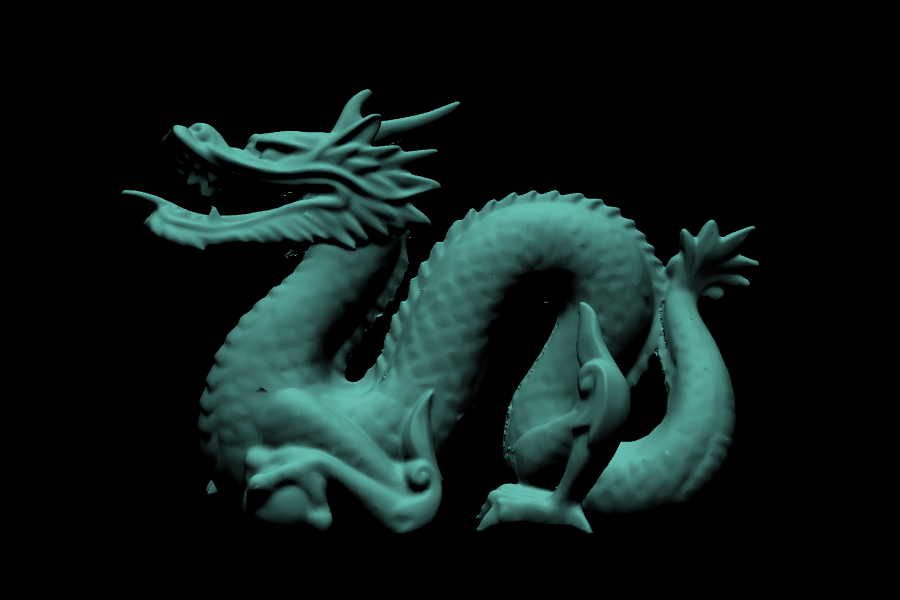
\includegraphics[width=\textwidth]{img/difuso}
   \caption{Difuso}
 \end{subfigure}
\\
 \begin{subfigure}[b]{0.42\textwidth}
   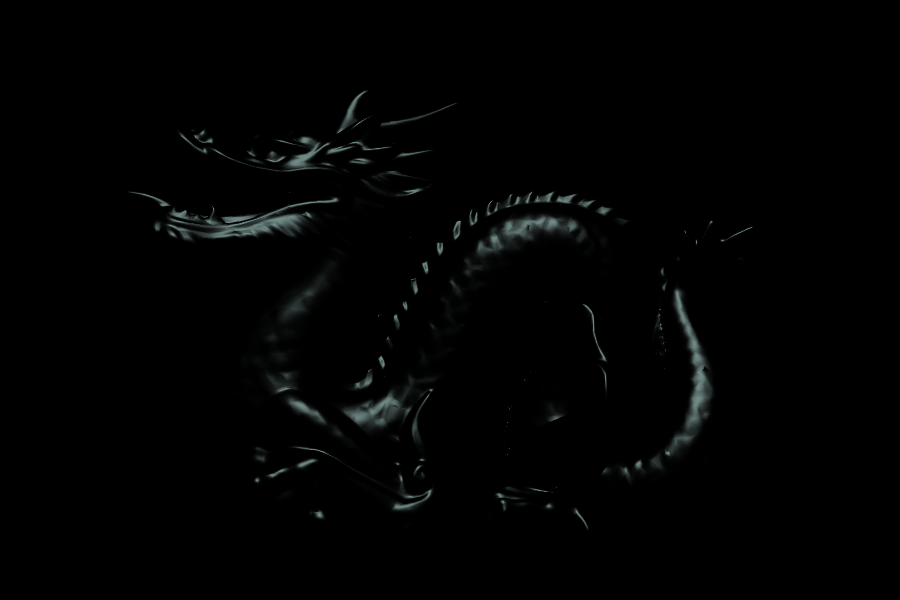
\includegraphics[width=\textwidth]{img/especular}
   \caption{Especular}
 \end{subfigure}
~
 \begin{subfigure}[b]{0.42\textwidth}
   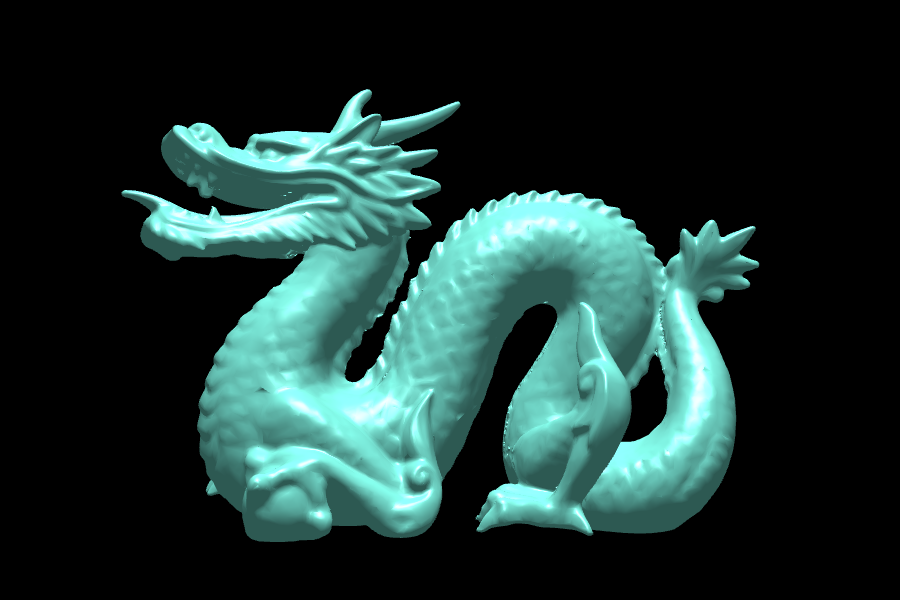
\includegraphics[width=\textwidth]{img/completo}
   \caption{Completo}
 \end{subfigure}
\end{figure} 
\end{columns}
\end{frame}

\begin{frame}{¿Cómo se calcula la reflexión?}
La reflexión de la luz (color) de un punto en la superficie se calcula como:
 $$\mathbf{L}_a \mathbf{k}_a + \mathbf{L}_d \mathbf{k}_d (\mathbf{n} \cdot \mathbf{l}) + \mathbf{L}_s \mathbf{k}_s (\mathbf{v} \cdot \mathbf{h})^{\alpha}$$
 En donde:
 \begin{itemize}
  \item $\mathbf{L}$ son los tres colores (ambiente, difuso y especular) de la luz.
  \item $\mathbf{k}$ son los tres colores (ambiente, difuso y especular) del material.
  \item $\alpha$ es la constante del brillo del material.
  \item $\mathbf{n}$ la normal a la superficie en el punto.
  \item $\mathbf{l}$ un vector unitario que apunta a la fuente de luz desde el punto.
  \item $\mathbf{v}$ un vector unitario que apunta a la camara desde el punto.
  \item $\mathbf{h} = \frac{\mathbf{l} + \mathbf{v}}{|\mathbf{l} + \mathbf{v}|}$ un vector unitario, llamado \say{halfway vector}.
 \end{itemize}
\end{frame}


\begin{frame}{Detalles de implementación}
\begin{itemize}
  \item A cada objeto de la escena se le asiga un material en vez de un color.
  \item En escenas simples, se aconseja definir la luz como blanco intenso; para evitar complicaciones.
   \item El material esta formado por tres colores $\mathbf{k}_a, \mathbf{k}_d, \mathbf{k}_s$ y un escalar ($\alpha$).
   \item Usualmente restringimos $\alpha \in [ 0.5, 128 ]$, y cuando experimenatmos, la variamos logaritmicamente.
  \begin{itemize}
   \item Un $\alpha$ grande produce brillos pequeños y concentrados.
   \item Un $\alpha$ pequeño produce brillos grandes y débiles.
  \end{itemize}
  \item Dado que no se puede \say{restar luz}, los productos puntos $\mathbf{n} \cdot \mathbf{l}$ y $\mathbf{v} \cdot \mathbf{h}$ deben ser no negativos.
  \item Si hay mas de una luz en la escena:
  \begin{itemize}
   \item Se calcula el componente ambiental una vez.
   \item Y los componentes difuso y especular una vez por cada luz, acumulando (sumando) el resultado,
  \end{itemize}
\end{itemize}
\end{frame}

\begin{frame}{Ejercicio: Mejorar el Ray Marching anterior}
\url{https://github.com/nemediano/tallerShadertoy/tree/main/codigo/Ejercicio5}
\begin{columns}
\column[t]{0.5\textwidth}
     \begin{itemize}
         \item Lógica para desplegar varios objetos en la escena, uno de ellos un piso.
         \item La cámara se define con el modelo LookAt. Idealmente una cámara que gire alrededor de la escena.
         \item Utilice el algoritmo de Blinn–Phong para hacer el shading
     \end{itemize}
\column[t]{0.5\textwidth}
        \begin{figure}[htb]
            \centering
            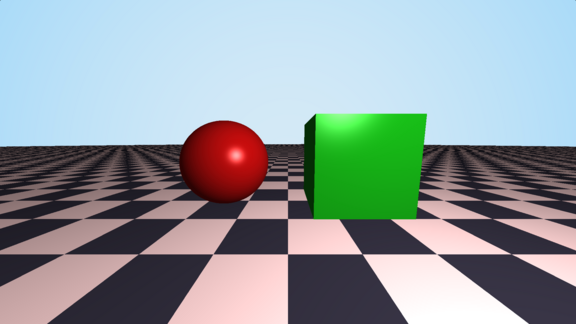
\includegraphics[width=0.6\textwidth]{img/Ejer/Ejer5}
        \end{figure}
\end{columns}
\end{frame}

\subsection{Modelado geométrico usando las sdf}

\begin{frame}{Transformaciones afines de 3D}
\begin{itemize}
    \item Las transformaciones afines se pueden generalizar a 3D.
    \item La traslación y el escalamiento se generalizan de manera trivial.
    \item La rotación en 3D, requiere de un parámetro extra: un \alert{vector} unitario que nos sirve de eje de rotación.
    \begin{itemize}
        \item La rotación sigue siendo con respecto al origen.
        \item Recuerda, que los vectores son libres en el espacio.
    \end{itemize}
    \item Aquí solo usaremos una función que nos devuelve la matriz de rotación a partir de un angulo y un vector.
    \item Puedes ver como se construye en el excelente libro: \href{https://mathweb.ucsd.edu/~sbuss/CourseWeb/Math155A_2019Winter/SecondEdDraft.pdf}{3D Computer Graphics: A mathematical approach with OpenGL}
    
\end{itemize}
\end{frame}

\begin{frame}[fragile]{Signed distance functions en 3D}
\begin{block}{¿Dónde puedo buscar mas sdf?}
    El mejor lugar para buscar una sdf es el \href{https://iquilezles.org/articles/distfunctions/}{sitio personal} de Inigo Quilez
\end{block}
Para aumentar el poder de expresividad, puedes pasar un parámetro extra que sea la transformación afín.
Para un cubo por ejemplo:
\begin{listing}
\begin{minted}{glsl}
float sdBox(vec3 position, vec3 boxCenter, vec3 boxSizes) {
  vec3 q = abs(position - boxCenter) - boxSizes;
  return length(max(q, 0.0)) + min(max(q.x, max(q.y, q.z)), 0.0);
}

float sdBox(vec3 position, mat4 T) {
  vec3 tPos = (inverse(T) * vec4(position, 1.0)).xyz;
  vec3 q = abs(tPos) - vec3(1.0);
  return length(max(q, 0.0)) + min(max(q.x, max(q.y, q.z)), 0.0);
}
\end{minted}
\end{listing}

\end{frame}

\begin{frame}{Deformando el espacio}

\begin{itemize}
    \item Escalar \alert{deforma el espacio} y eso afecta las funciones de distancia.
    \item El Ray Marching es mas tolerable a expandir el espacio que a contraer el espacio. Es decir, es \alert{posible} que escalar por números mayores que uno funcione.
    \item Algunas sdf pueden escalarse directamente desde la formula. La Figura muestra una caja (cubo) escalado en: $(\frac{1}{2}, 1, \frac{1}{2})$ por ambos métodos.
\end{itemize}

\begin{figure}[htp]
 \centering
 \begin{subfigure}[b]{0.22\textwidth}
   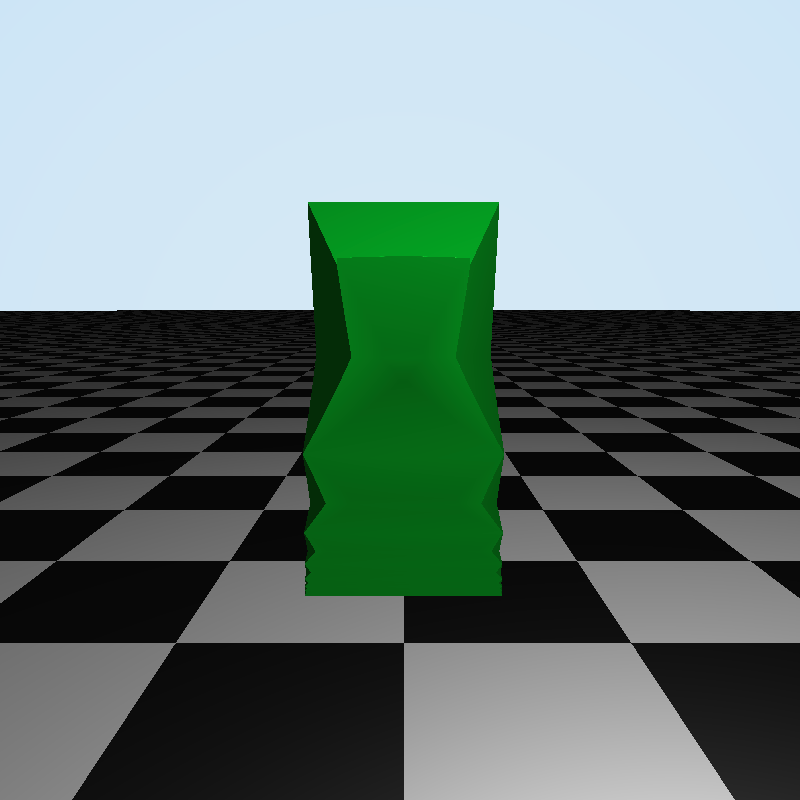
\includegraphics[width=\textwidth]{img/inestable}
   \caption{Matriz}
 \end{subfigure}
~
 \begin{subfigure}[b]{0.22\textwidth}
   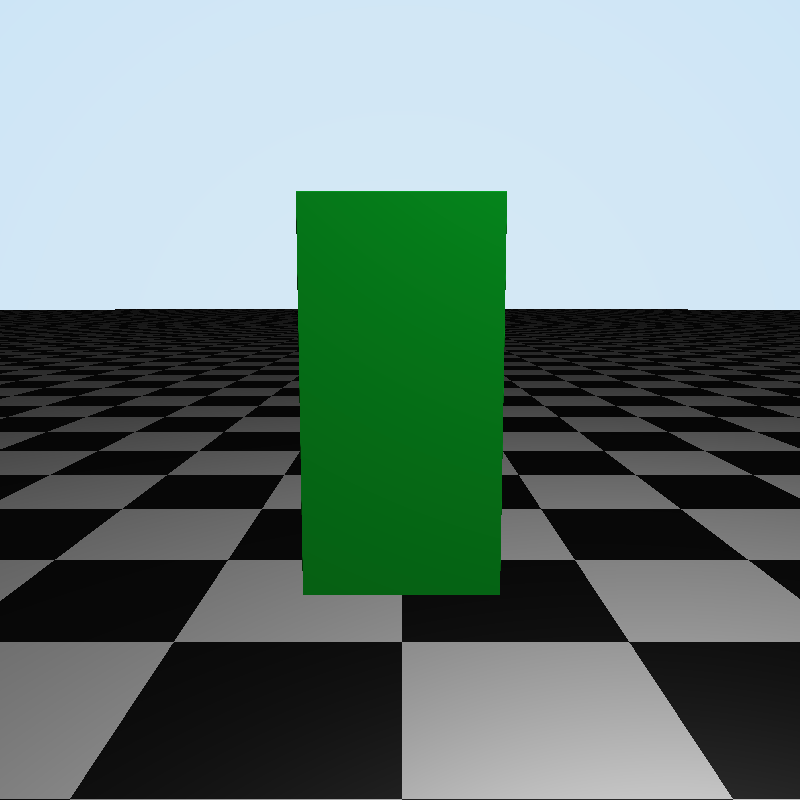
\includegraphics[width=\textwidth]{img/estable}
   \caption{Formula}
 \end{subfigure}
\end{figure} 

\end{frame}

\begin{frame}{Constructive Solid Geometry}

\begin{columns}
\column[t]{0.5\textwidth}
\begin{itemize}
    \item La \href{https://en.wikipedia.org/wiki/Constructive_solid_geometry}{Constructive solid geometry} (CSG) es una forma de hacer modelado geométrico.
    \item Se usan operaciones como unión, intersección, y diferencia.
    \item Esta técnica es particularmente apropiada para usarse con Ray Marching y sdfs.
\end{itemize}
\column[t]{0.5\textwidth}
        \begin{figure}[htb]
            \centering
            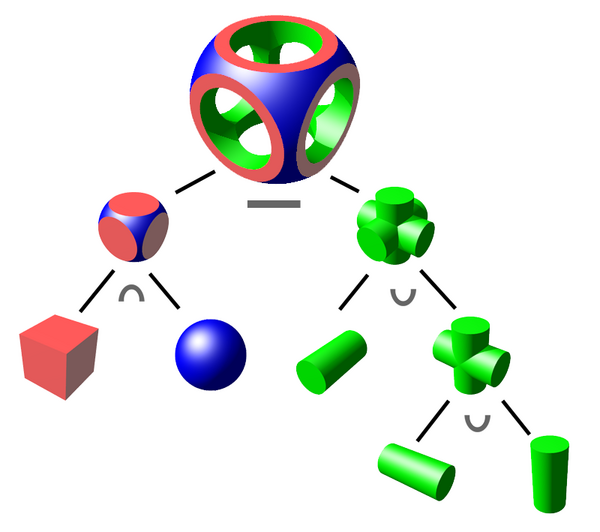
\includegraphics[width=0.6\textwidth]{img/cgsTree}
        \end{figure}
\end{columns}

\end{frame}

\begin{frame}[fragile]{¿Cómo lo podemos usar nosotros?}
Cuando usamos Ray Marching basado en sdf, prácticamente tenemos todo lo necesario.
\begin{listing}
\begin{minted}{glsl}
float opUnion(float lhsd, float rhsd) {
    return min(lhsd, rhsd);
}

float opSubtraction(float lhsd, float rhsd) {
    return max(-lhsd, rhsd);
}

float opIntersection(float lhsd, float rhsd) {
    return max(lhsd, rhsd);
}
\end{minted}
\end{listing}
Donde \mintinline{glsl}{lhs} y \mintinline{glsl}{rhs}, son las sdf de las dos formas a combinar.
\end{frame}

\begin{frame}[fragile]{Operaciones booleanas suaves}
\begin{listing}
\begin{minted}{glsl}
float opSmoothUnion(float lhsd, float rhsd, float smoothFactor) {
    float h = clamp(0.5 + 0.5 * (rhsd - lhsd) / smoothFactor, 0.0, 1.0);
    return mix(rhsd, lhsd, h) - smoothFactor * h * (1.0 - h);
}

float opSmoothSubtraction(float lhsd, float rhsd, float smoothFactor) {
    float h = clamp(0.5 - 0.5 * (rhsd + lhsd) / smoothFactor, 0.0, 1.0);
    return mix(rhsd, -lhsd, h) + smoothFactor * h * (1.0 - h);
}

float opSmoothIntersection(float lhsd, float rhsd, float smoothFactor) {
    float h = clamp(0.5 - 0.5 * (rhsd - lhsd) / smoothFactor, 0.0, 1.0);
    return mix(rhsd, lhsd, h) + smoothFactor * h * (1.0 - h);
}

\end{minted}
\end{listing}
Donde \mintinline{glsl}{smoothFactor} es un factor (medido en la unidades de distancia de la escena), que nos dice cuanto hay que \alert{dilatar} el resultado de la operación.
\end{frame}

\begin{frame}[fragile]{Ejemplo: diferencia y la diferencia suave}
\begin{listing}
\begin{minted}{glsl}
float sdCompousedShape(vec3 position) {
    float sphereDis = sdSphere(position, vec3(0), 1.0);
    float boxDis = sdBox(position, vec3(0.5, 0.0, 0.0), vec3(0.8));  
    return opSmoothSubtraction(sphereDis, boxDis, 0.15);
}
\end{minted}
\end{listing}

\begin{figure}[htp]
 \centering
\begin{subfigure}[b]{0.2\textwidth}
   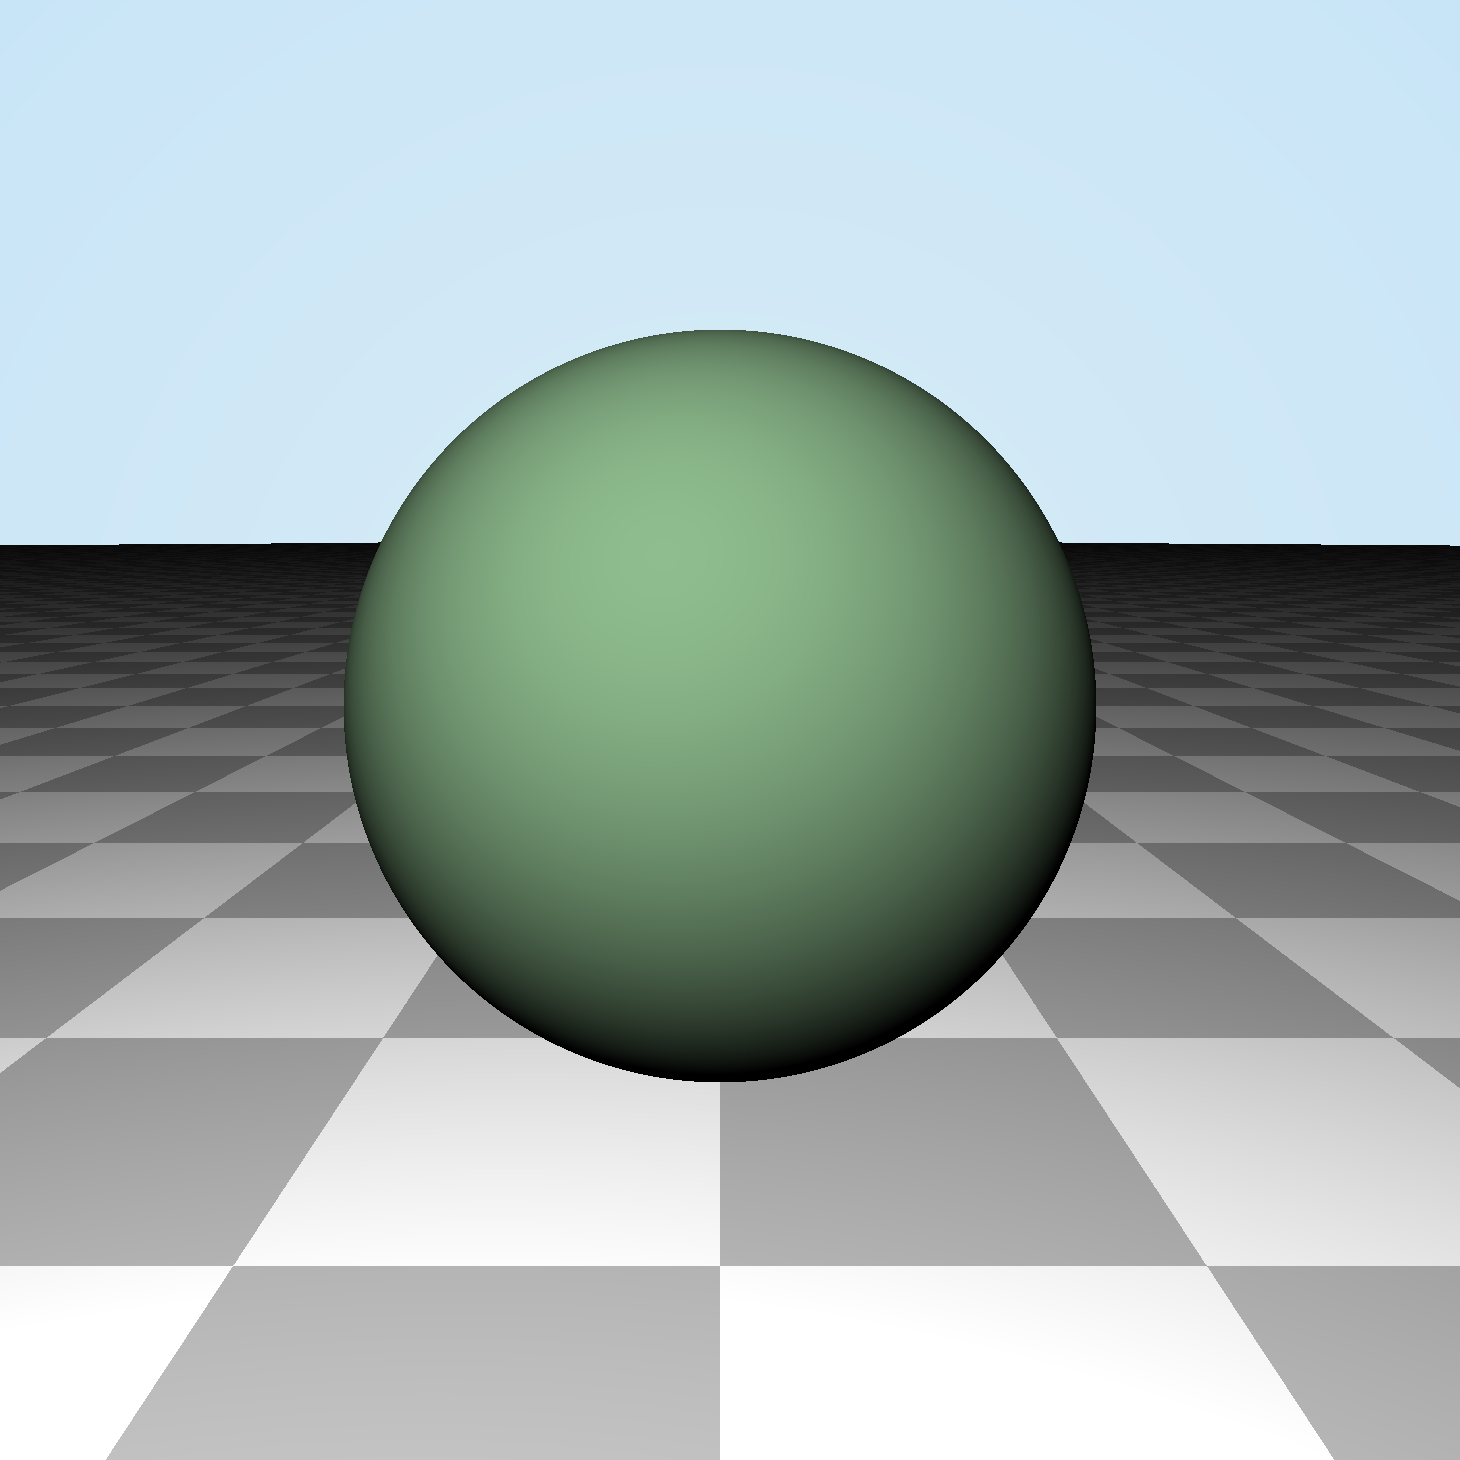
\includegraphics[width=\textwidth]{img/RightSphere}
   \caption{Esfera}
 \end{subfigure}
~
 \begin{subfigure}[b]{0.2\textwidth}
   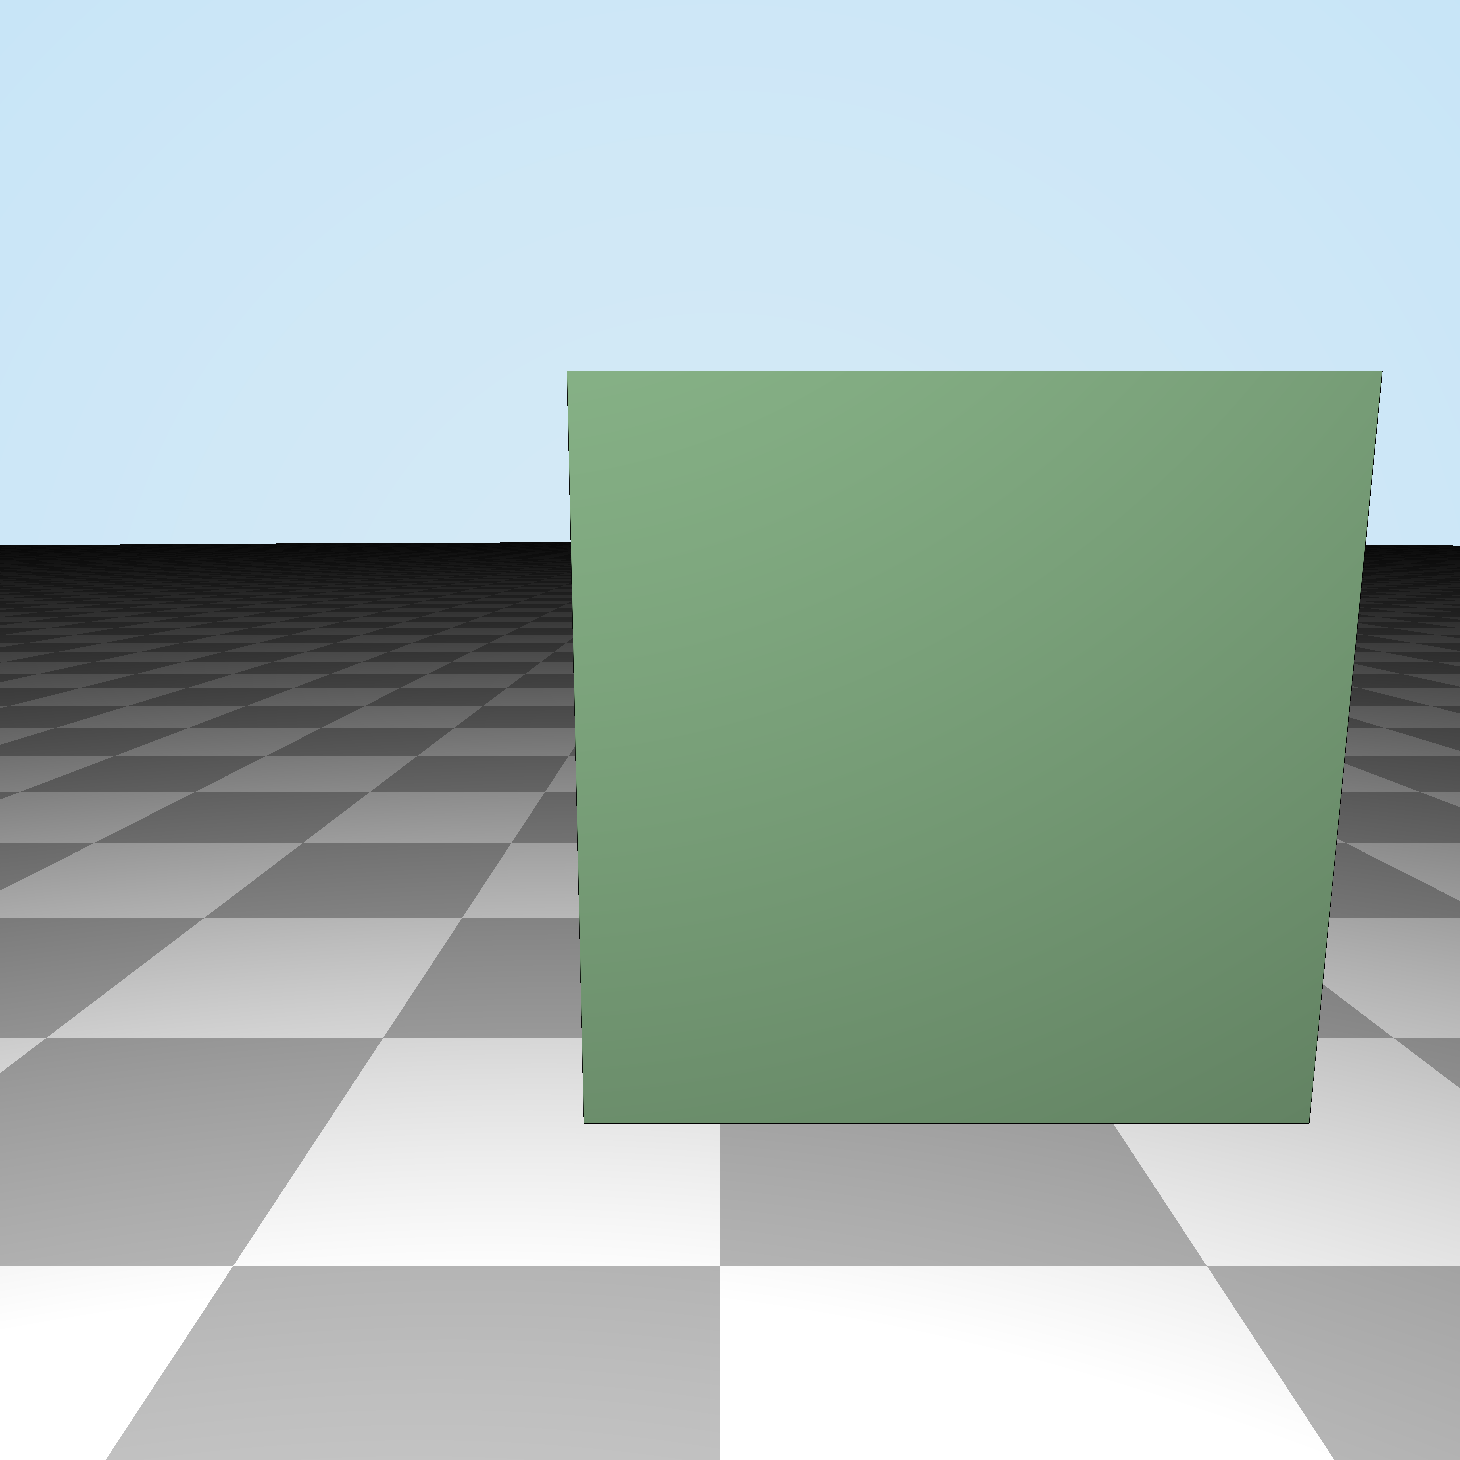
\includegraphics[width=\textwidth]{img/leftBox}
   \caption{Cubo}
 \end{subfigure}
~
 \begin{subfigure}[b]{0.2\textwidth}
   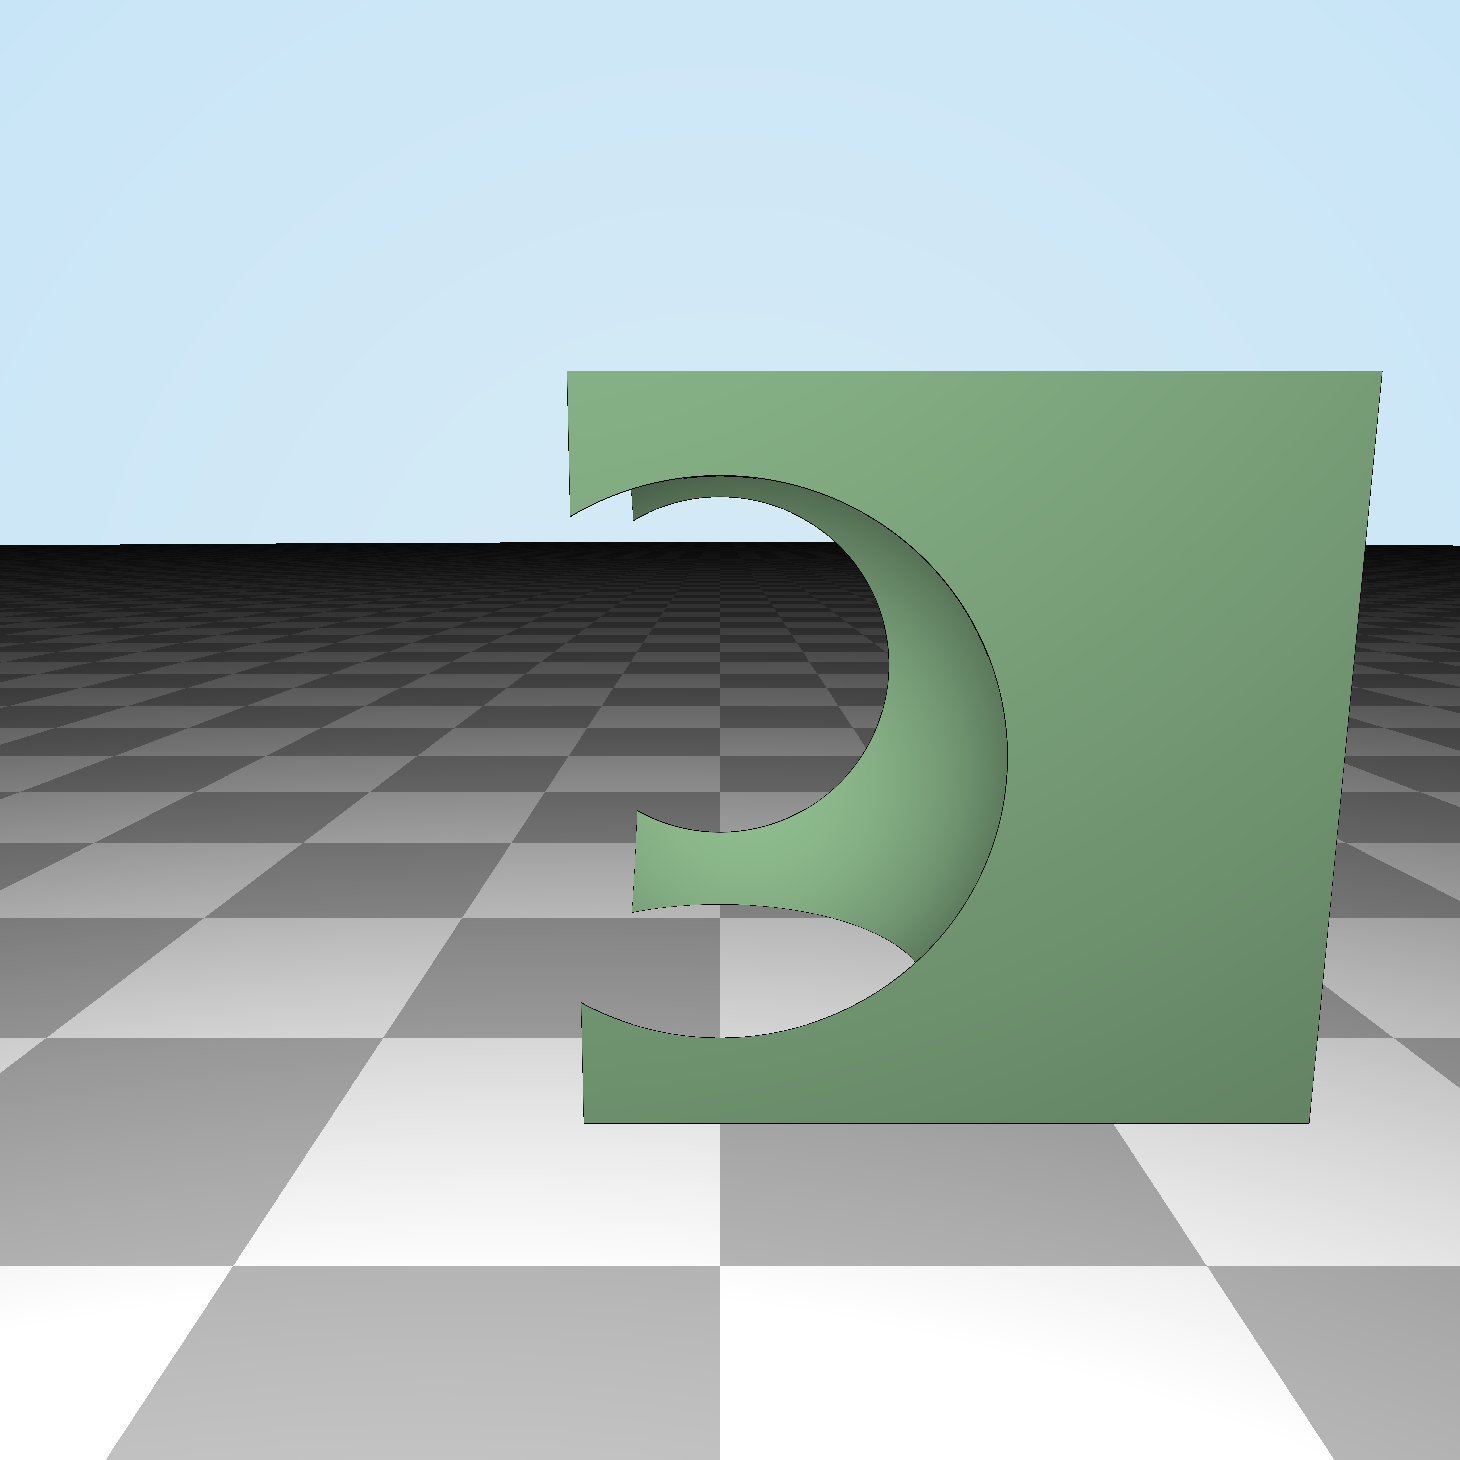
\includegraphics[width=\textwidth]{img/Substraction}
   \caption{Diferencia}
 \end{subfigure}
~
 \begin{subfigure}[b]{0.2\textwidth}
   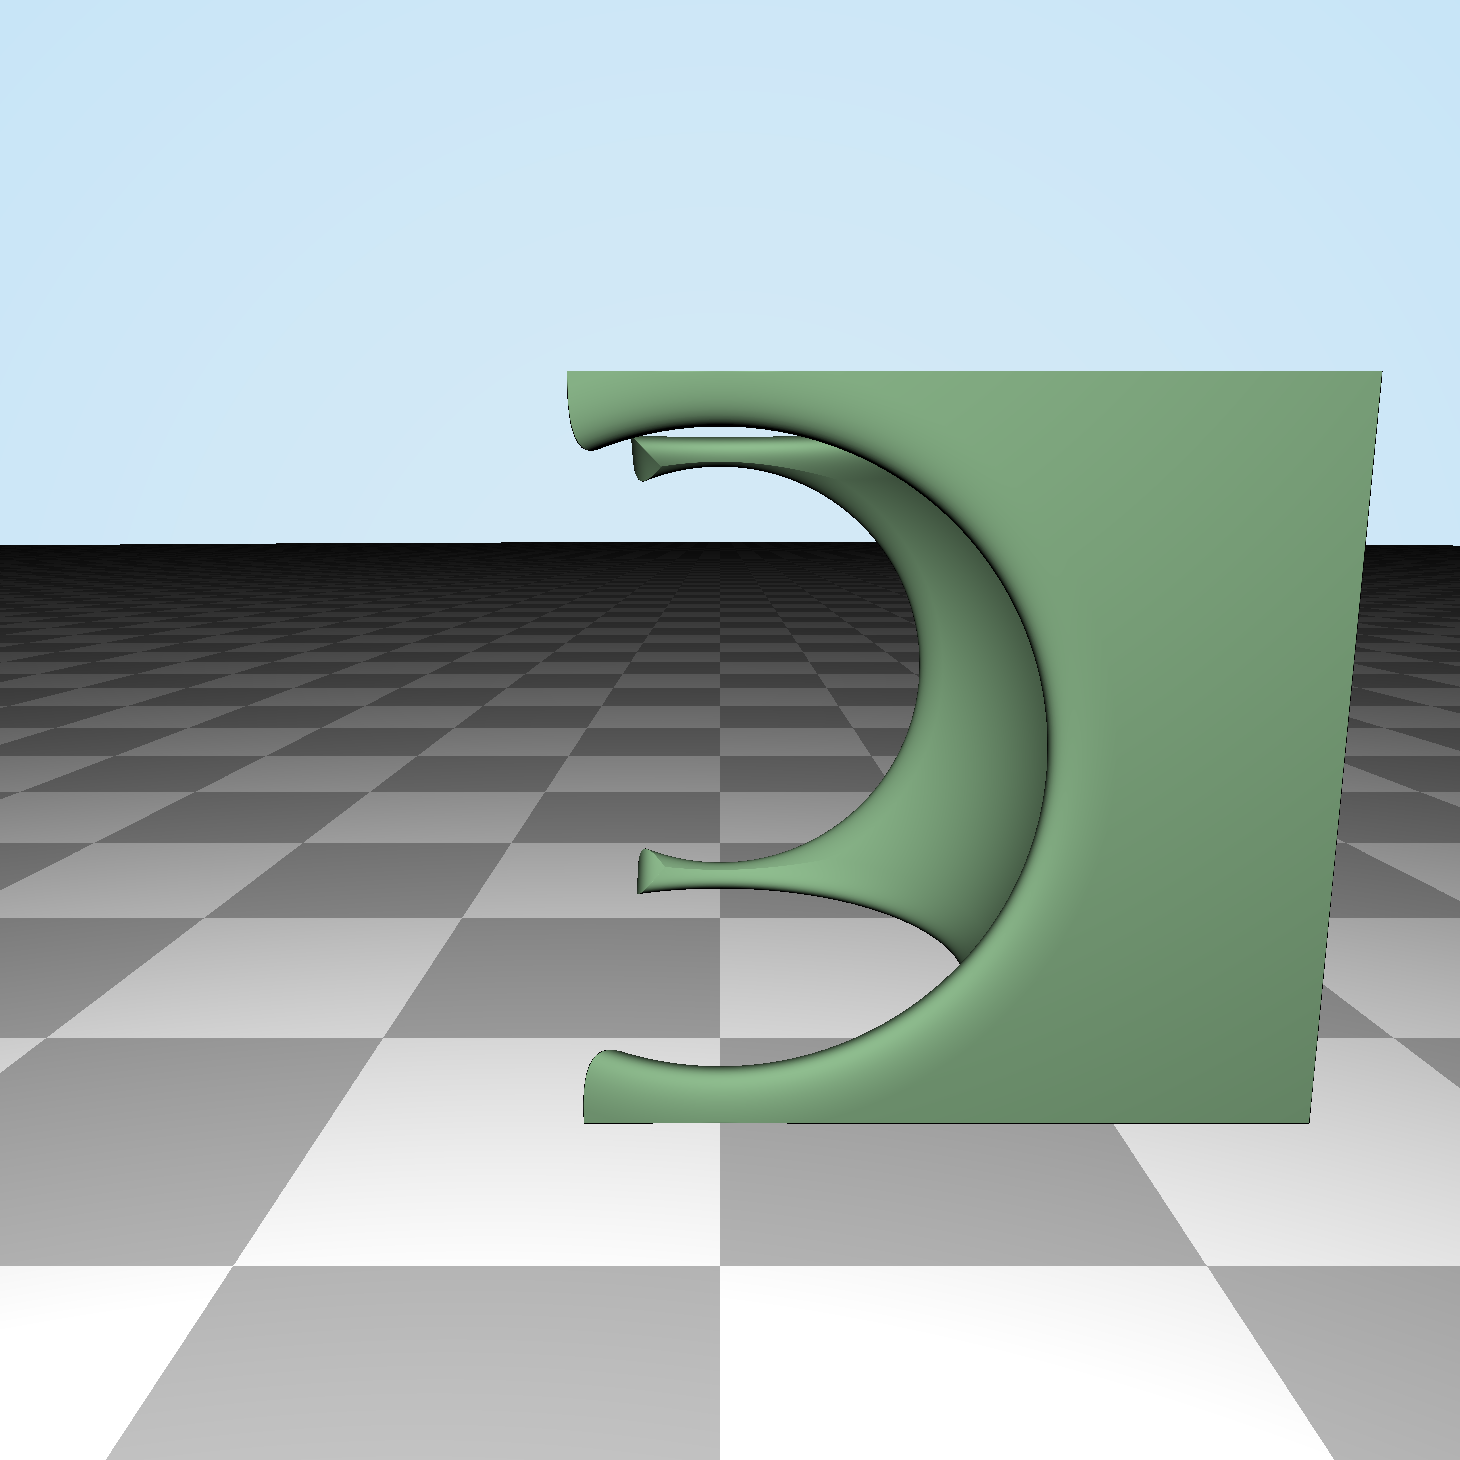
\includegraphics[width=\textwidth]{img/SmoothSubstraction}
   \caption{Diferencia suave: $0.15$}
 \end{subfigure}
\end{figure}
\end{frame}

